% ch2p11_001: Clipping a path
% rectangular and circular
\documentclass[tikz, border=10pt]{standalone}

\usepackage{tikz}

\begin{document}
	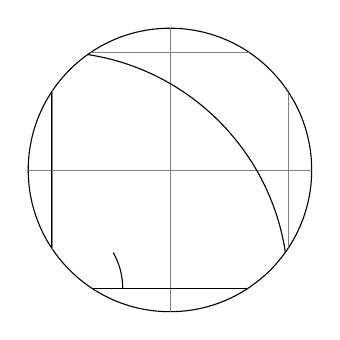
\begin{tikzpicture}[scale=3]
		% rectangular
		% \clip (-0.1, -0.2) rectangle (1.1, 0.75);
		
		% circular
		% \clip (0, 0) circle (0.85cm);
		
		% Or a better way (is to draw)
		% \clip[draw] (0, 0) circle (0.6);  % Clip has border now
		
		% Another option
		\draw[clip] (0.5, 0.5) circle [radius=0.6cm];
		
		\draw[step=0.5, gray, very thin] (-1.4, -1.4) grid (1.4, 1.4);
		\draw (-1.5, 0) -- (1.5, 0);    % x-axis
		\draw (0, -1.5) -- (0, 1.5);    % y-axis
		
		\draw (0, 0) circle [radius=1cm];
		\draw (3mm, 0mm) arc [start angle=0, end angle=30, radius=3mm];
	\end{tikzpicture}
\end{document}